\documentclass[dvipdfmx, xcolor=svgnames]{beamer}

\usetheme{Madrid}
\setbeamertemplate{navigation symbols}{}
\setbeamertemplate{footline}[frame number]
\setbeamertemplate{footline}[section]
\usepackage{graphicx}
\usepackage{amsmath}
\usepackage{amssymb}
\usepackage{txfonts}
\usepackage{tabularx}
\usepackage{color}
\usepackage{colortbl}
\usepackage{centernot}
%\mathversion{bold}
\renewcommand{\familydefault}{\sfdefault}
\renewcommand{\kanjifamilydefault}{\gtdefault}
\setbeamerfont{title}{size=\large,series=\bfseries}
\setbeamerfont{frametitle}{size=\large,series=\bfseries}
%\setbeamerfont{framesubtitle}{size=\small,series=\bfseries}
\setbeamercolor{title}{fg=white, bg=Navy}
\setbeamertemplate{frametitle}[default][left]
\setbeamercolor{frametitle}{fg=white, bg=Navy}
%\setbeamercolor{framesubtitle}{fg=white, bg=black} %%%%%%%%%% 反映されないよ
\usefonttheme{professionalfonts}

\usepackage[deluxe]{otf}
\usepackage[noalphabet]{pxchfon}
\setboldgothicfont{HaranoAjiGothic-Medium.otf}

\theoremstyle{plain}
%\setbeamertemplate{theorems}
%\newtheorem{main}{Main Result}
\newtheorem{thm}{Theorem}[section]
\newtheorem{cor}{Corollary}[section]
\newtheorem{prop}{Proposition}[section]
\newtheorem{lemm}{Lemma}[section]
\theoremstyle{definition}
\newtheorem*{defi}{Definition}
%\newtheorem{fact}{Fact}[section]
\newtheorem{question}{Question}
\newtheorem{exam}{Example}[section]
\newtheorem{assumption}{Assumption}[section]
%\numberwithin{equation}{section}
\theoremstyle{remark}
\newtheorem{remark}{Remark}[section]


\usepackage{amsmath,amssymb,amsthm,amscd,ascmac,mathrsfs,bm,type1cm,multirow,array,enumerate,mathrsfs,tabularx}
\usepackage{wrapfig,float}
% \usepackage{graphicx}
\usepackage{color}
\usepackage{arydshln} % 行列 c:c 
% \usepackage[dvipdfmx]{graphicx}

\renewcommand{\arraystretch}{1.1}

\renewcommand{\theenumi}{\arabic{enumi}}

\newcounter{main} % カウンタの宣言
\setcounter{main}{0} % カウンタの初期化
\resetcounteronoverlays{main}
\newcommand{\useMain}[1][]{\refstepcounter{main}{#1}Main Result \,{\themain}}


\newcounter{Prop} % カウンタの宣言
\setcounter{Prop}{0} % カウンタの初期化
\resetcounteronoverlays{Prop}
\newcommand{\useProp}[1][]{\refstepcounter{Prop}{#1}Proposition \,{\theProp}}



\def\rnum#1{\expandafter{\romannumeral #1}} 
\def\Rnum#1{\uppercase\expandafter{\romannumeral #1}} 
\def\hsymb#1{\mbox{\strut\rlap{\smash{\Huge$#1$}}\quad}} % 行列の省略記号*

\newcommand{\BigFig}[1]{\parbox{12pt}{\Huge #1}}
\newcommand{\BigZero}{\BigFig{0}} 


\setcounter{tocdepth}{1}


\title{模擬授業(20分)}
\author{東京理科大学理学研究科 \quad
        小林 穂乃香}
%\institute{小池研究室}
\date{山口大学面接\, 於\\
      2022年9月5日}

\begin{document}
%%%%% page 1 (title page) %%%%%
\frame{\titlepage}


\section{1. ユークリッド幾何学とリーマン幾何学}

\frame{
\frametitle{\insertsection}
{\large {\bf 今まで習ってきた幾何学は,全てユークリッド幾何学}}\vspace{5pt}

\hspace{20pt} \(\cdots\)“\underline{真っ直ぐな物差し}”が定義された真っ直ぐな空間

\hspace{43pt} {\small (ユークリッド計量)}\vspace{8pt}
\pause
\begin{itemize}
\item \(X=(X_1, \ldots, X_n), \,\, Y=(Y_1, \ldots, Y_n) \,\, \in \mathbb{R}^n, \)
      \begin{table}
      \begin{tabular}{lll}
      \(\langle \, , \, \rangle\) : \textcolor{red}{{\it \(\mathbb{R}^n\)上のユークリッド計量}}
      & \(\overset{\mathrm{def}}{\Leftrightarrow}\)
      & \(\langle X, Y\rangle =\sum_{i=1}^n X_iY_i\)
      \end{tabular}
      \end{table}
\vspace{5pt}

\item \((\mathbb{R}^n, \langle \, ,\, \rangle )\)を\textcolor{red}{ユークリッド空間}という
\end{itemize}
\vspace{20pt}
\pause

{\large {\bf リーマン幾何学では,空間や計量が真っ直ぐとは限らない}}\vspace{5pt}

\hspace{20pt} \(\cdots\)リーマン多様体とは,\underline{リーマン計量}が定義された多様体のこと

}




\frame{
\frametitle{\insertsection}
\hspace{3pt}\(M\) \hspace{4pt}: \(C^\infty\)多様体 
\vspace{3pt}

\(T_p M\) : 点\(p\in M\)における\(M\)の接空間
\vspace{3pt}

\( X, Y \,\in T_pM\)
\vspace{5pt}
\begin{itemize}
\item  \(g : T_p M \times T_p M \rightarrow \mathbb{R}\)
      \vspace{-0pt}
            \begin{table}
                  \begin{tabular}{llcl}
                        \hspace{-10pt}\(g\) : \textcolor{red}{{\it \(M\)上のリーマン計量}}
                        & \(\overset{\mathrm{def}}{\Leftrightarrow}\)
                        & (\rnum{1})& \(g\) : 双線型
                        \\
                        & & (\rnum{2})& \(g( X, Y)=g(Y, X)\)(対称)
                        \\
                        & &
                        (\rnum{3})& \(g(X, X)\geq 0\) かつ\\
                        & & &\(g(X, X)=0\Leftrightarrow X=0\)(正定値)
                        \end{tabular}
            \end{table}
      \vspace{5pt}
\item このとき,組\((M, g)\)を\textcolor{red}{リーマン多様体}という
\end{itemize}
\vspace{20pt}
\pause

\(\mathbb{R}^n\)は\(C^\infty\)多様体であり,ユークリッド計量はリーマン計量である
\vspace{10pt}

\raisebox{-0.5mm}[0mm]{
\includegraphics[bb=0 0 150 30, scale=0.5]{yokoyazirushi.png}} \hspace{-40pt}
{\bf \underline{ユークリッド空間\((\mathbb{R}^n, \langle \, ,\, \rangle )\)はリーマン多様体のひとつ}}
}





\section{2. なぜ曲がった空間を考えるのか}

\frame{
\frametitle{\insertsection}
\underline{例1.} \quad 東京--ニューデリー間の最短距離は?
\begin{center}
\scalebox{0.13}{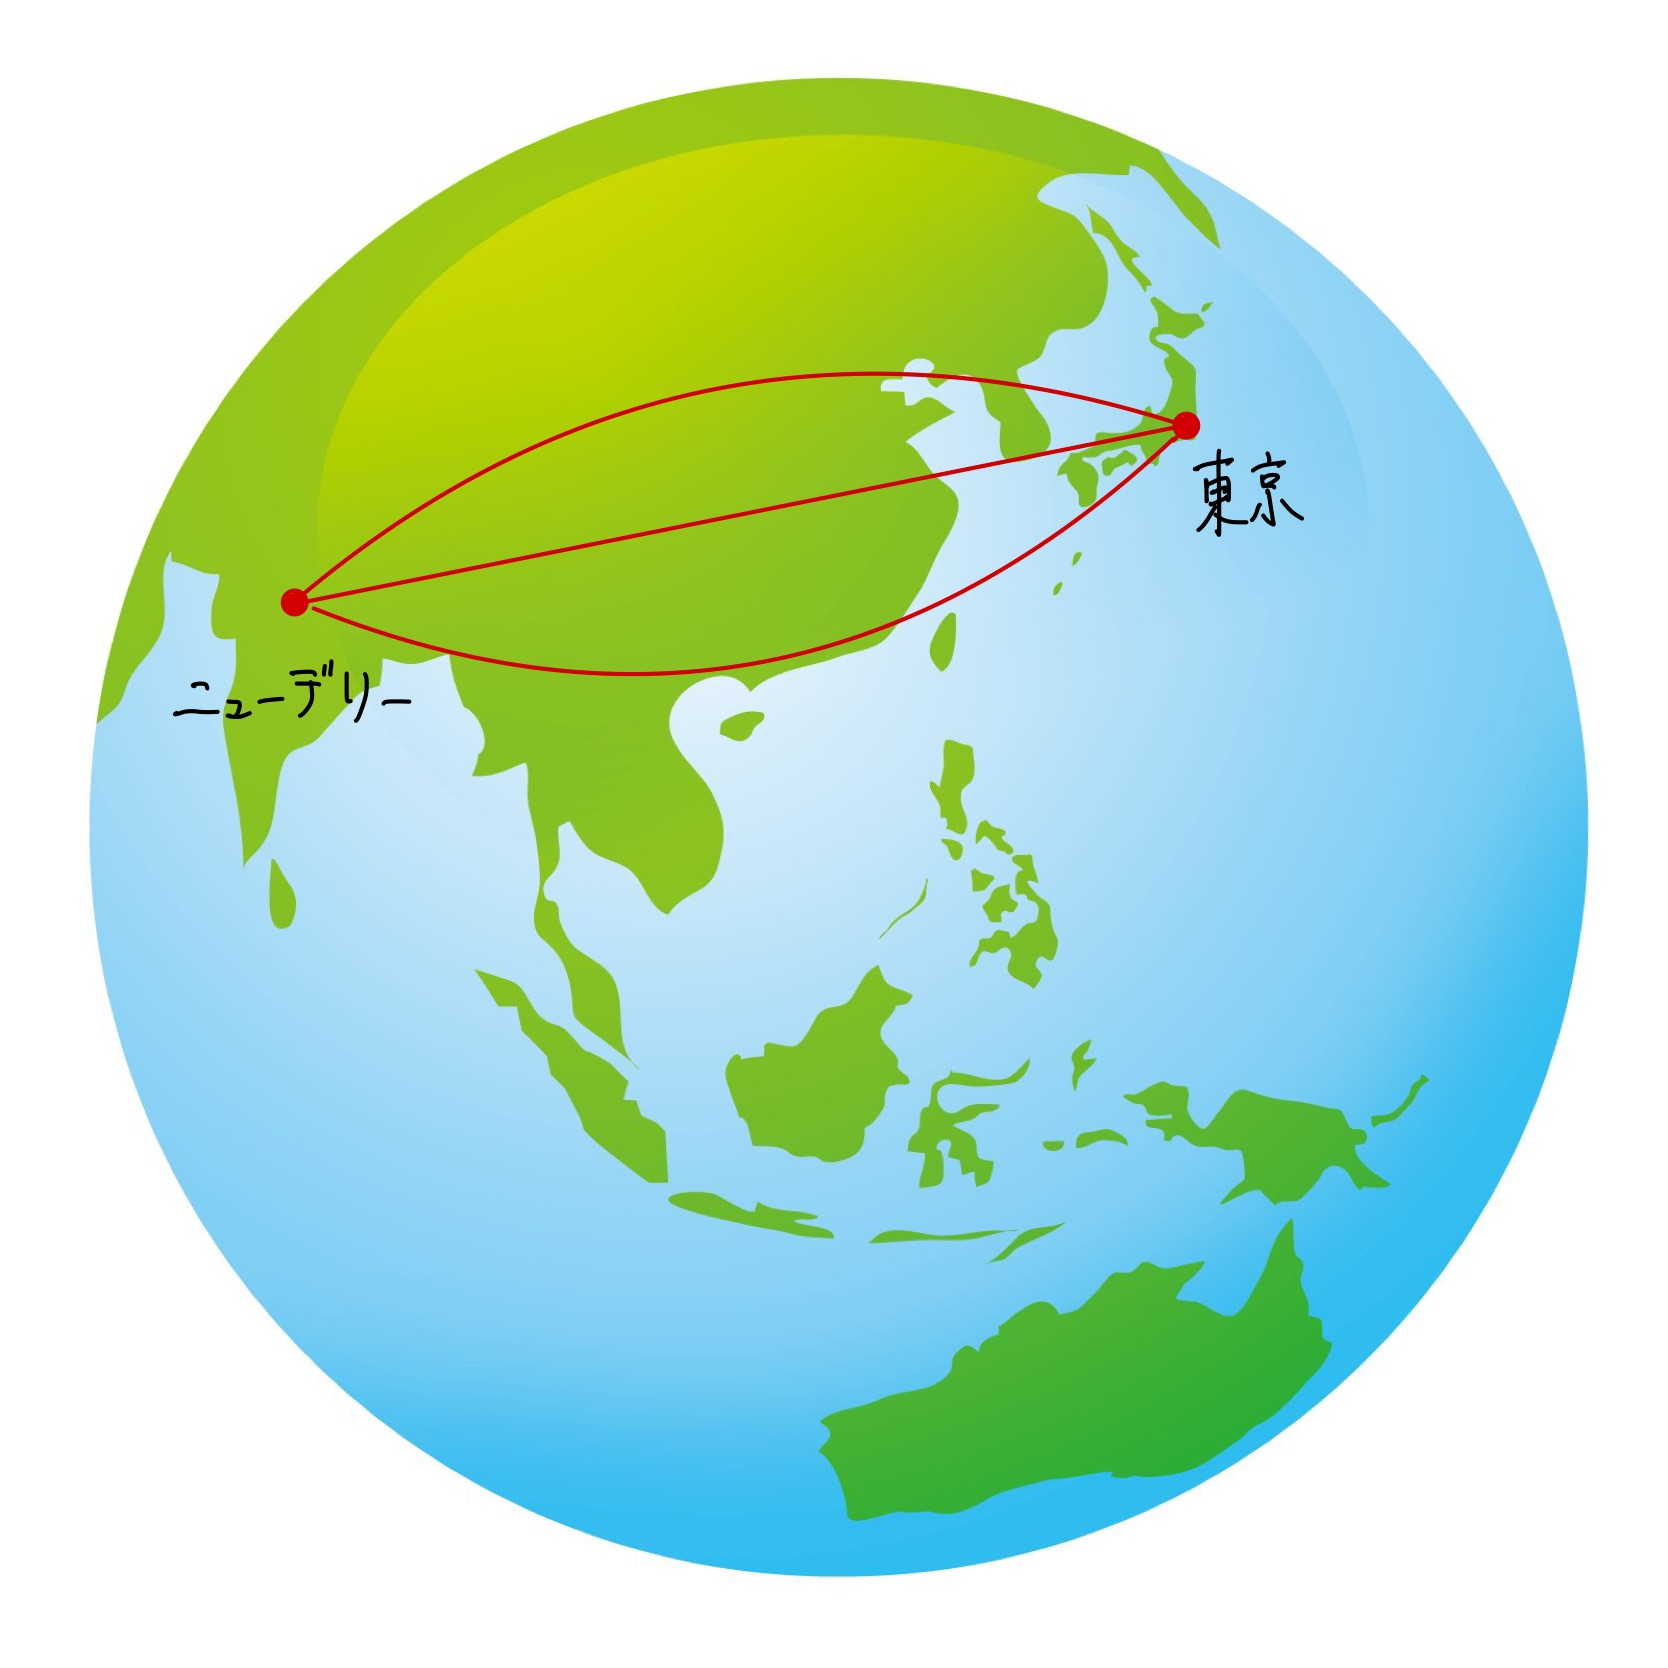
\includegraphics{chikyuugi2.jpg}}
\end{center}
}



\frame{
\frametitle{\insertsection}
\underline{例2.} \quad 重力場における光の軌跡
\vspace{-5pt}
\begin{center}
\only<1>{
\scalebox{0.25}{
\includegraphics{logoRikadai.png}}
}
\only<2>{
\scalebox{0.13}{
\includegraphics{logoRikadai2.jpg}} 
}      
\only<3->{
\scalebox{0.13}{
\includegraphics{logoRikadai3.jpg}} 
}      
\end{center}
\pause
{\bf \underline{aの位置にある天体が,b地点から見える(重力レンズ効果)}}
\pause
\begin{itemize}
      \item 光は常に“真っ直ぐ”進む
      \item 重力によって歪んだ空間では\(c_1\)が“直線”
\pause
      \item \(c_2\)が直線に見えるのは,我々は無意識のうちにこの世界を
      
            ユークリッド空間として見ているから
\end{itemize}
}





\frame{
\frametitle{\insertsection}
\underline{例3.} \quad \(\mathbb{R}^n\)における非ユークリッド計量
\vspace{10pt}

\(X =\{(x_1, x_2)\in \mathbb{R}^2\, |\, x_2 >0\}\)上のリーマン計量\(g\)を,次のように定義する:
\vspace{-5pt}

\[g(\bm{v}, \bm{w}) := \dfrac{1}{x_2^2}\langle \bm{v}, \bm{w}\rangle \quad \quad (\bm{v}, \bm{w} \in T_p X,\,\, p \in X)\]
\vspace{3pt}

\pause
問.\((X, g)\)上の曲線\(c_i\)の長さを求めよ.
\[c_1(t)=(t, 1), \,\,\, c_2(t)=(t, 2), \,\,\, c_3(t)=(1, t), \,\,\, c_4(t)=(1, 2t) \]
\pause
\vspace{-10pt}
\begin{defi}
曲線 \(c : [a, b] \rightarrow (M, g)\)の長さ\(L_g(c)\)は次のように定義される:
\vspace{-5pt}
\[
\begin{aligned}
\Vert \dot{c}(t)\Vert_g &:= \sqrt{g(\dot{c}(t), \dot{c}(t))} \vspace{-3pt}\\
L_g(c)&:= \int_{a}^{b} \Vert \dot{c}(t)\Vert_g \,dt \vspace{10pt}
\end{aligned}
\]
\vspace{-5pt}
\end{defi}
}



\frame{
\frametitle{\insertsection}
\[c_1(t)=(t, 1), \,\,\, c_2(t)=(t, 2), \,\,\, c_3(t)=(1, t), \,\,\, c_4(t)=(1, 2t)\]
\begin{center}
      \scalebox{0.2}{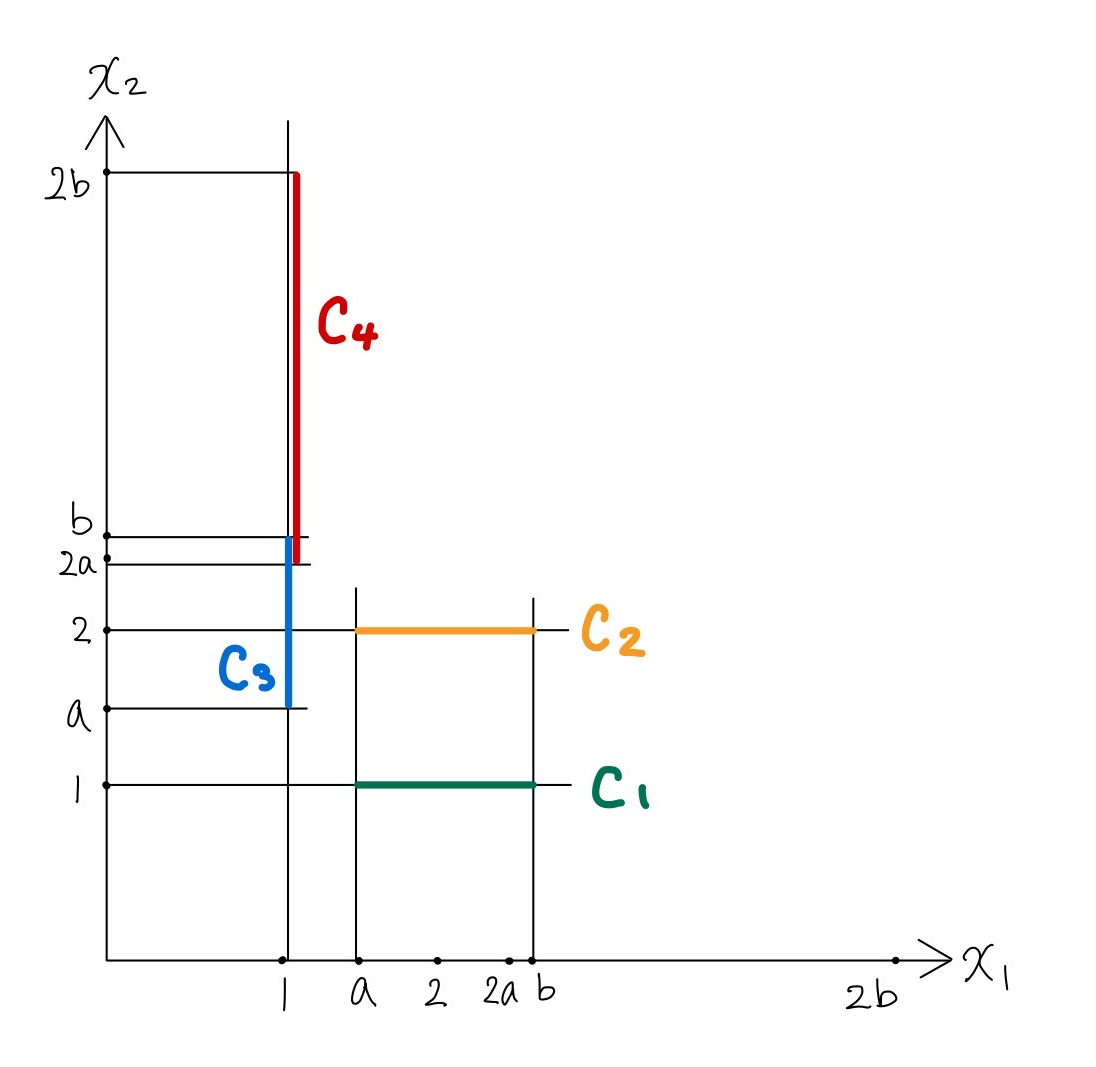
\includegraphics{mensetsu-metric.png}}
\end{center}
}


\frame{
\frametitle{\insertsection}
\begin{table}
      \vspace{-10pt}
\begin{tabular}{lc}
\begin{minipage}{0.55\textwidth}
\begin{itemize}
  \item \(c_1(t)=(t, 1), \,\,\dot{c}_1(t)=(1, 0)\)
        \vspace{3pt}
        
        \(g(\dot{c}_1(t), \dot{c}_1(t)) = \dfrac{1}{1^2}\langle \dot{c}_1(t), \dot{c}_1(t)\rangle =1\)
        \vspace{-5pt}
        \[\therefore \, L_g(c_1) = \int_{a}^{b} dt = \textcolor{MediumSeaGreen}{\underline{b-a}}\]
        \vspace{-5pt}
        
        \uncover<2->{
  \item \(c_2(t)=(t, 2),\,\, \dot{c}_2(t)=(1, 0)\)
        \vspace{3pt}
        
        \(g(\dot{c}_2(t), \dot{c}_2(t)) = \dfrac{1}{2^2}\langle \dot{c}_2(t), \dot{c}_2(t)\rangle =\dfrac{1}{2^2}\)
        \vspace{-5pt}
        \[\therefore \, L_g(c_2) = \int_{a}^{b} \dfrac{1}{2}dt = \textcolor{DarkOrange}{\underline{\dfrac{1}{2}(b-a)}}\]
        }
\end{itemize}
\end{minipage}
&
\uncover<1->{
\begin{minipage}{0.45\textwidth}
      \begin{center}
            \scalebox{0.14}{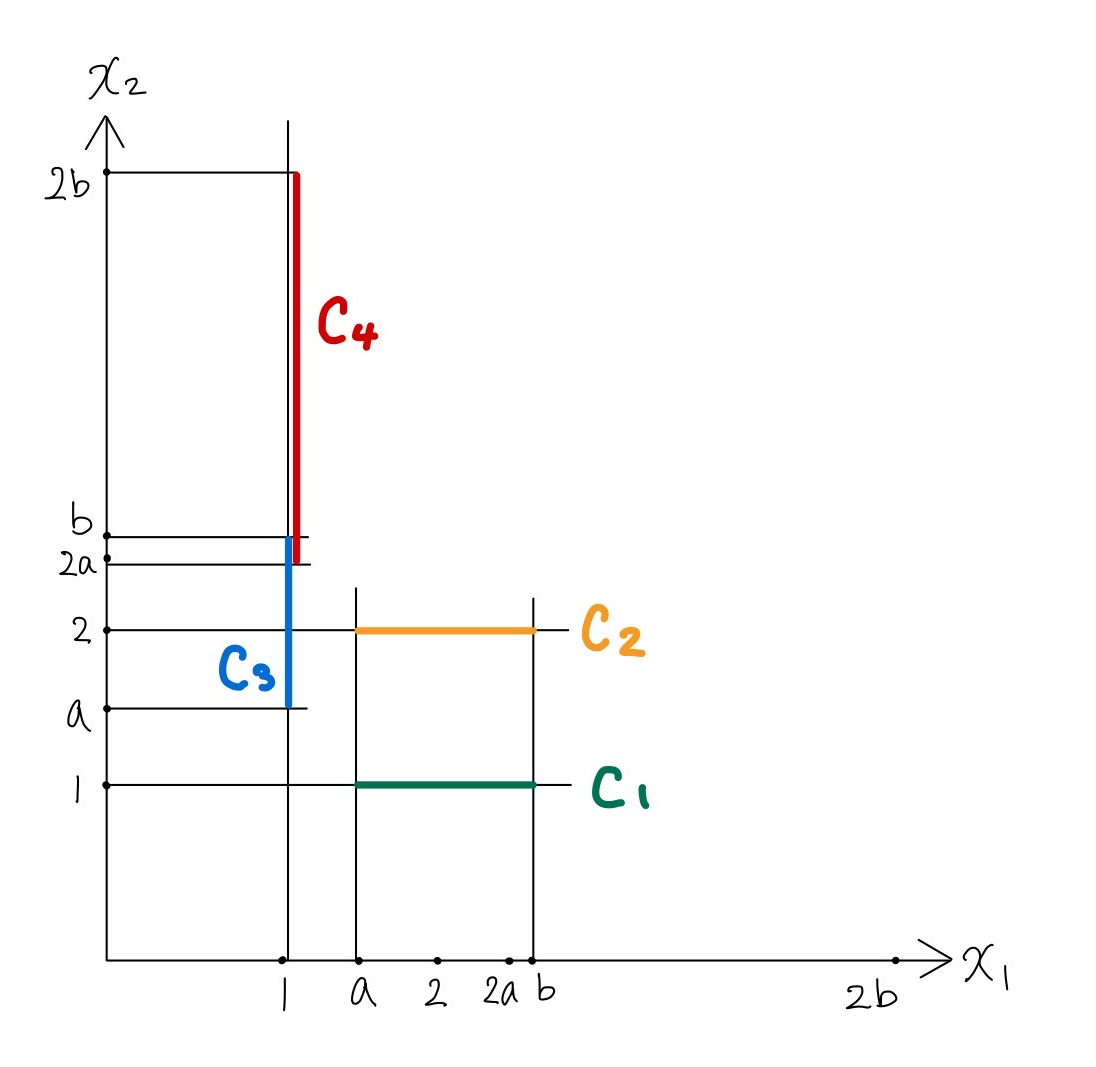
\includegraphics{mensetsu-metric.png}}
      \end{center}
      % \scalebox{0.2}{
\includegraphics{logoRikadai.png}}
\end{minipage}
}
\end{tabular}
\vspace{5pt}
\end{table}
\uncover<3->{
\raisebox{-0.5mm}[0mm]{
\includegraphics[bb=0 0 150 30, scale=0.5]{yokoyazirushi.png}} \hspace{-40pt}
{\bf ユークリッド空間では\(c_1\)と\(c_2\)の長さは同じだが,}\vspace{3pt}

\hspace{42pt} {\bf \((X, g)\)上では異なる!}
}

}




\frame{
\frametitle{\insertsection}
\begin{table}
      \vspace{-10pt}
\begin{tabular}{lc}
\begin{minipage}{0.55\textwidth}
\begin{itemize}
  \item \(c_3(t)=(1, t), \,\, \dot{c}_3(t)=(0, 1)\)
        \vspace{3pt}
        
        \(g(\dot{c}_3(t), \dot{c}_3(t)) = \dfrac{1}{t^2}\)
        \vspace{-5pt}
        \[\therefore \, L_g(c_3) = \int_{a}^{b} \dfrac{1}{t}dt = \textcolor{RoyalBlue}{\underline{\log \dfrac{b}{a}}}\]
        \vspace{-5pt}
  \item \(c_4(t)=(1, 2t), \,\, \dot{c}_4(t)=(0, 2)\)
        \vspace{3pt}
        
        \(g(\dot{c}_4(t), \dot{c}_4(t)) = \dfrac{1}{t^2}\)
        \vspace{-5pt}
        \[\therefore \, L_g(c_4) = \int_{a}^{b} \dfrac{1}{t}dt = \textcolor{red}{\underline{\log \dfrac{b}{a}}}\]
\end{itemize}
\end{minipage}
&
\begin{minipage}{0.45\textwidth}
      \begin{center}
            \scalebox{0.14}{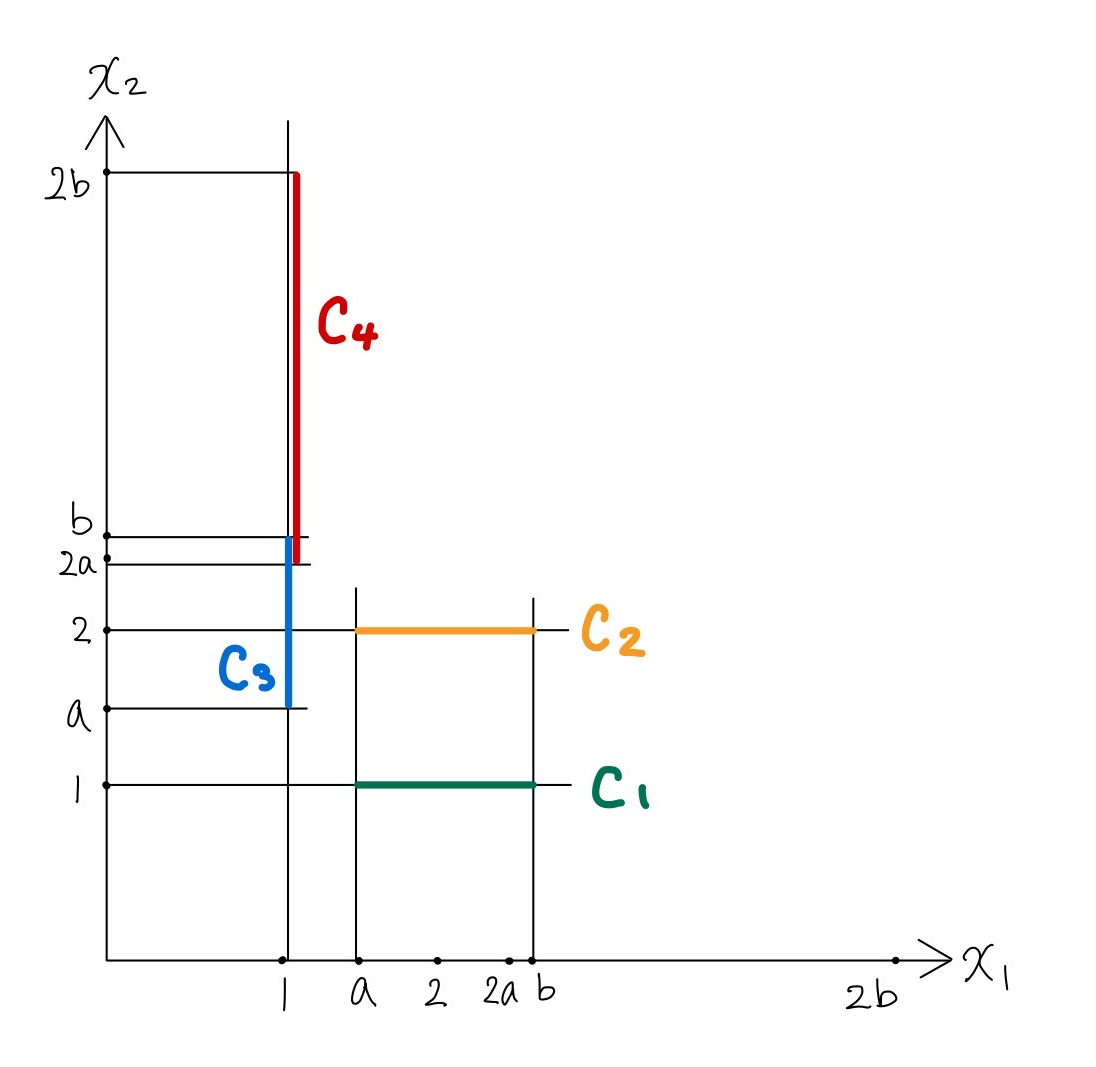
\includegraphics{mensetsu-metric.png}}
      \end{center}
      % \scalebox{0.2}{
\includegraphics{logoRikadai.png}}
\end{minipage}
\end{tabular}
\vspace{5pt}
\end{table}
\pause
\raisebox{-0.5mm}[0mm]{
\includegraphics[bb=0 0 150 30, scale=0.5]{yokoyazirushi.png}} \hspace{-40pt}
{\bf ユークリッド空間では\(c_3\)と\(c_4\)の長さは異なるが,}\vspace{3pt}

\hspace{42pt} {\bf \((X, g)\)上では同じ長さ!}

}




\section{3. 曲がった空間における“真っ直ぐ”とは?}


\frame{
\frametitle{\insertsection}
\begin{table}
      \vspace{-10pt}
\begin{tabular}{ccc}
ユークリッド空間における直線
&
\(\cdots\)
&
2階微分がゼロ
\vspace{3pt}
\\
\raisebox{-2mm}[0mm]{
\includegraphics[width=12pt, height=18pt, scale=0.2]{yazirusitate.png}} 
{\small 拡張}
&
&
\vspace{3pt}
\\
リーマン多様体における\textcolor{red}{測地線}
&
\(\cdots\)
&
2階微分がゼロ
\end{tabular}
\end{table}
\pause
まずは,曲がった空間における微分を定義する.
\begin{defi}
\hspace{4pt}\(M\)\hspace{3pt} : \(C^\infty\)多様体\vspace{3pt}

\(TM\) : \(M\)の接束
\vspace{-15pt}
\begin{table}
      \begin{tabular}{llcl}
      \(\nabla : TM \times TM \rightarrow TM\) : \textcolor{red}{{\it \(M\)の接続}}
      & \(\overset{\mathrm{def}}{\Leftrightarrow}\)
      & (\rnum{1})& \(\nabla_{fX+Y}Z=f\nabla_X Z +\nabla_Y Z\)
      \\
      & & (\rnum{2})& \(\nabla_X (aY+Z)=a\nabla_X Y +\nabla_X Z\)
      \\
      & &
      (\rnum{3})& \(\nabla_X (fY)=X(f)Y+f\nabla_X Y\)
      \end{tabular}
      \end{table}
ここで,\(X, \, Y,\, Z \, \in TM, \,\, f \in C^\infty(M),\,\, a \in \mathbb{R}.\)
\vspace{5pt}

\(\nabla_X Y\)を,\(X\)についての\(Y\)の\textcolor{red}{共変微分}という.
\end{defi}
}





\frame{
\frametitle{\insertsection}
\begin{thm}
リーマン多様体\((M, g)\)に対して,次を満たすような接続\(\nabla\)は唯一定まる:
\begin{table}
\begin{tabular}{cl}
(\rnum{4}) & \([X, Y]=\nabla_X Y -\nabla_Y X\)\\
(\rnum{5}) & \(Xg(Y, Z)=g(\nabla_X Y, Z) +g(Y , \nabla_X Z)\)
\end{tabular}
\end{table}
ここで,\(X,\, Y,\, Z\, \in TM.\)
\vspace{5pt}

(\rnum{1})〜(\rnum{5})を満たす接続\(\nabla\)を,\textcolor{red}{\(M\)のLevi-Civita接続}という.
\vspace{3pt}
\end{thm}
\begin{defi}
\(c\) : \((M, g, \nabla)\)上の\(C^\infty\)曲線
\vspace{-5pt}
\begin{table}
      \begin{tabular}{lll}
      \(c\) : \textcolor{red}{{\it \(M\)上の測地線}}
      & \(\overset{\mathrm{def}}{\Leftrightarrow}\)
      & \(\nabla_{\dot{c}}\dot{c}=0\)
      \end{tabular}
\end{table}
\end{defi}
}





\frame{
\frametitle{\insertsection}
実際に\(\nabla_{\dot{c}}\dot{c}\)を計算するために,いくつか準備をする.
\begin{defi}
\((M, g, \nabla)\) : \(n\)次元リーマン多様体, \,\,
\((x_1, \ldots, x_n)\) : \(M\)の座標
\vspace{5pt}

\(\partial_i :={\partial}/{\partial x_i}\) とする.
\[\nabla_{\partial_i} \partial_j =\sum_{k=1}^n \Gamma_{ij}^k\,\partial_k\]
によって定義される\(\Gamma_{ij}^k\)を,\textcolor{red}{\(\nabla\)の接続係数}という.
\end{defi}
\begin{prop}
\((M, g, \nabla)\)がユークリッド空間のとき,\(\Gamma_{ij}^k=0\)     
\end{prop}
}




\frame{
\frametitle{\insertsection}
\begin{prop}
      \((M, g, \nabla)\) : \(n\)次元リーマン多様体, \,\,
      \((x_1, \ldots, x_n)\) : \(M\)の座標
      \vspace{3pt}

      \(c : [a, b] \rightarrow M\) : \(M\)上の\(C^\infty\)曲線
      \vspace{3pt}

      とする.このとき,\vspace{-3pt}
      \[\nabla_{\dot{c}}\dot{c}=\sum_{k=1}^n \left( \frac{d^2(x_k\circ c)}{dt^2}+\sum_{i,j=1}^n \Gamma_{ij}^k \frac{d(x_i\circ c)}{dt}\frac{d(x_j\circ c)}{dt}\right)\frac{\partial}{\partial x_i}\]

      ここで,\(x_i \circ c\)は\(c\)の第\(i\)成分.
\end{prop}
\begin{corollary}
      \((M, g, \nabla)\)がユークリッド空間のとき,\(\Gamma_{ij}^k=0\)
      \vspace{-5pt}
      \begin{table}
      \begin{tabular}{lll}
      \(\therefore \quad \nabla_{\dot{c}}\dot{c}=0\)
      &
      \(\Leftrightarrow\)
      &
      \(\dfrac{d^2(x_k\circ c)}{dt^2}=0\) \vspace{3pt}
      \\
      &
      \(\Leftrightarrow\)
      & 
      \(c(t)=at+b \quad (a, b \in \mathbb{R})\)
      \end{tabular}
      \end{table}
      \vspace{-7pt}
\end{corollary}
}

\frame{
\frametitle{\insertsection}
\begin{corollary}
\(M \subset \mathbb{R}^n\)のとき
\[\left( \nabla_{\dot{c}}\dot{c}\right)_t=\mathrm{pr}_{\left(Tc(t)\right)}\left(\frac{d^2c}{dt^2}\right)\]
ここで,\(\mathrm{pr}_{\left(Tc(t)\right)}\)は\(c(t)\)の接空間\(T_{c(t)}M\)への直交射影.
\end{corollary}
}



\section{4. 球面における測地線}

\frame{
\frametitle{\insertsection}
\(S^2 \subset \mathbb{R}^3\)を考える.
\vspace{10pt}

\underline{問.} 
\begin{itemize}
\item \(c_1(t)=(\cos t, \sin t, 0)\)
\item \(c_2(t)=(\frac{1}{\sqrt{2}}\cos t, \frac{1}{\sqrt{2}}\sin t, \frac{1}{\sqrt{2}})\)
\vspace{3pt}
\end{itemize}
\(c_1, \, c_2\)は\(S^2\)の測地線か?

\begin{center}
\scalebox{0.1}{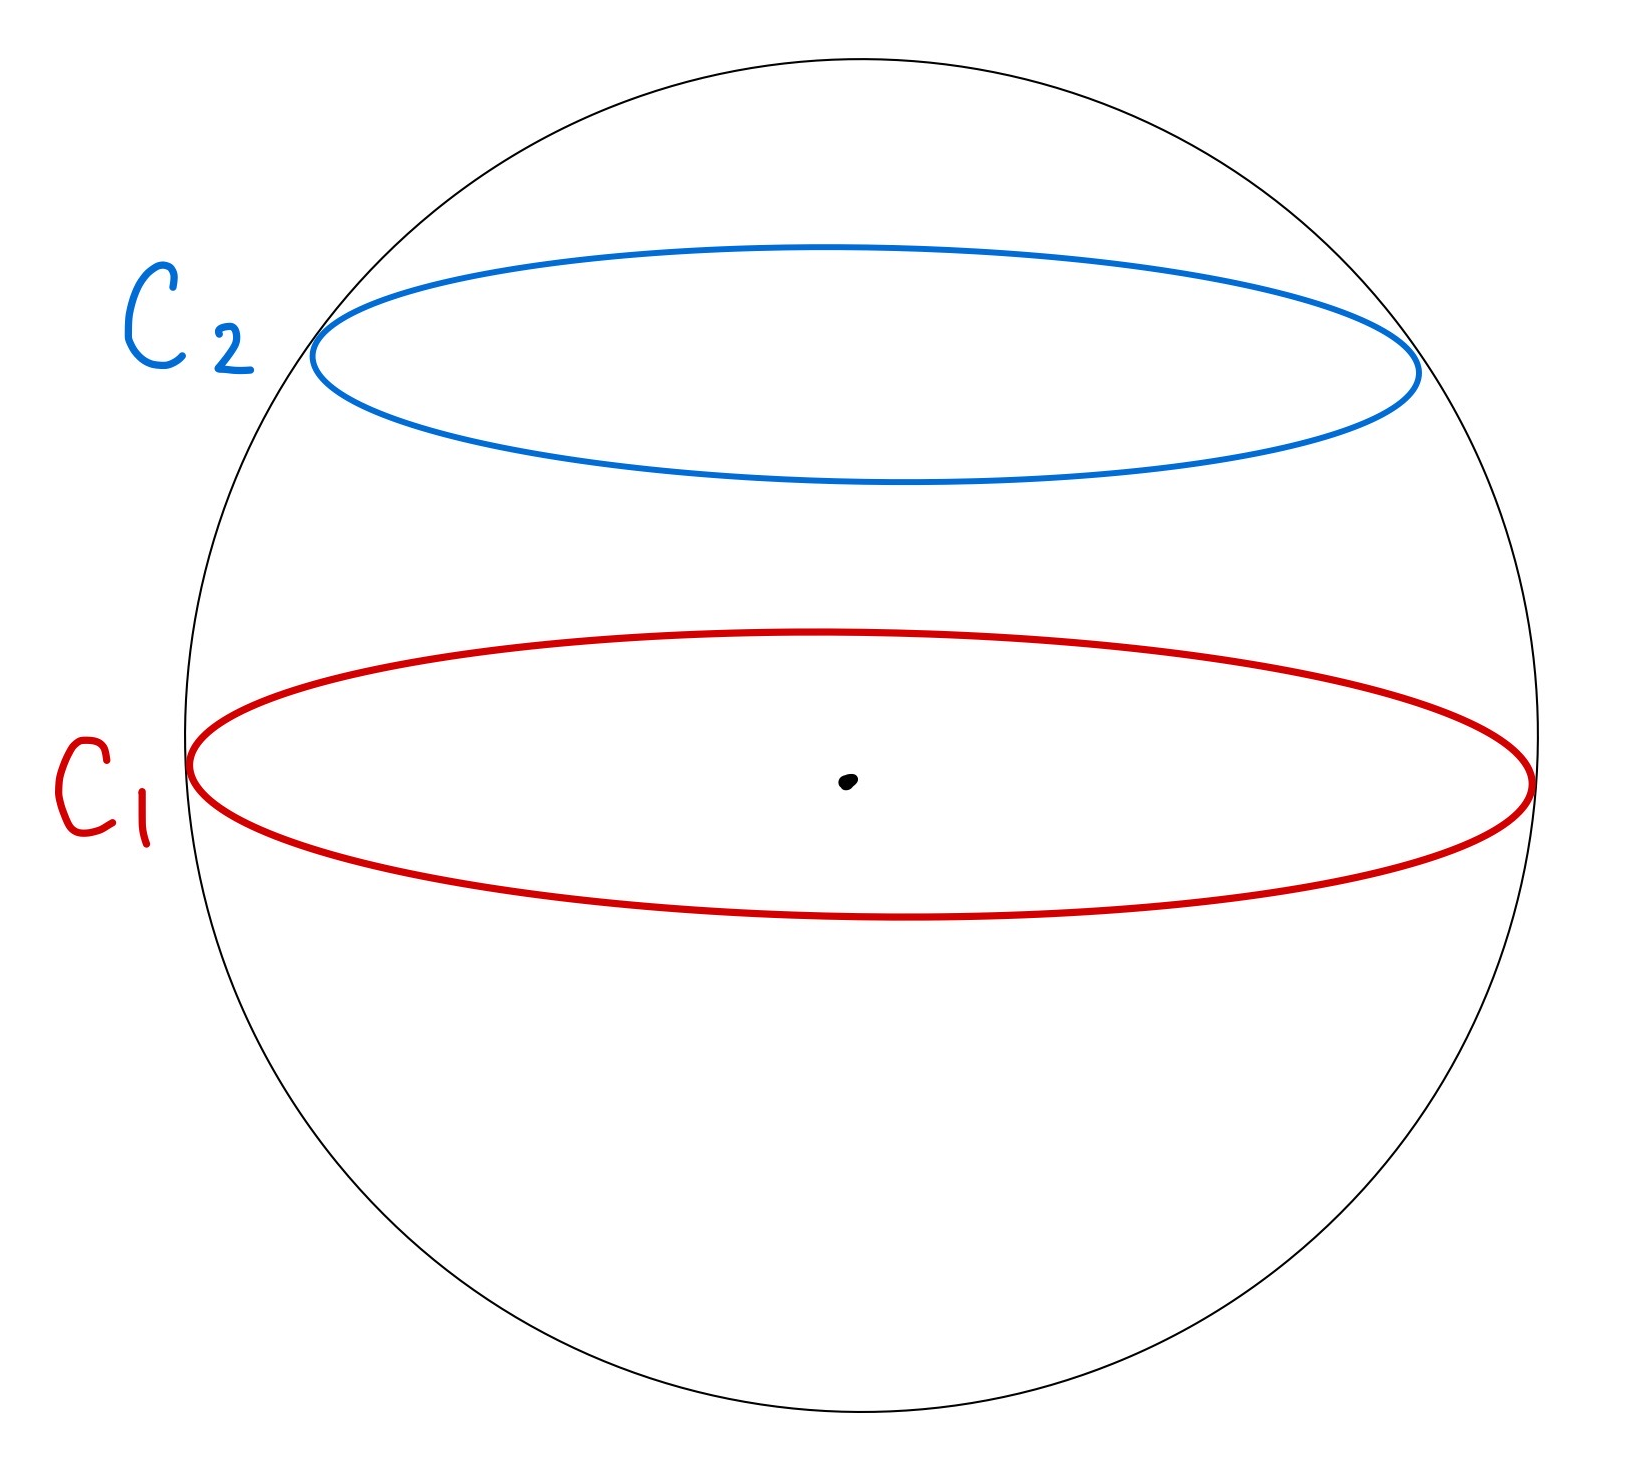
\includegraphics{mensetsu-mondai.png}}
\end{center}
}





\frame{
\frametitle{\insertsection}
\begin{prop}
\(S^n \subset \mathbb{R}^{n+1}\)の場合,
\vspace{-5pt}
\begin{center}
点\(c(t)\)における\(S^n\)の単位法ベクトル \(N_{c(t)}\)\quad \(=\)\quad 位置ベクトル\(c(t)\)
\end{center}
\end{prop}
\pause
\begin{table}
      \vspace{-10pt}
\begin{tabular}{l|r}
\begin{minipage}{0.48\textwidth}
\begin{itemize}
\item \underline{\(c_1(t)=(\cos t, \sin t, 0)\)}
\end{itemize}
\vspace{3pt}
        \[
        \begin{aligned}
            \left( \nabla_{\dot{c}_1}\dot{c}_1\right)_t&=\mathrm{pr}_{\left(T c_1(t)\right)}\left(\frac{d^2c_1}{dt^2}\right)\\
            &=\mathrm{pr}_{\left(T c_1(t)\right)}(-\cos t, -\sin t, 0)\\   
        N_{c_1(t)}&=c_1(t)\\
                  &=(\cos t, \sin t, 0)
        \end{aligned}
        \]
        \vspace{-5pt}
        \[\therefore \, \left(\nabla_{\dot{c}_1}\dot{c}_1\right)_t=\mathrm{pr}_{\left(T c_1(t)\right)}(-N_{c_1(t)})=0\]
        \begin{center}
        \(\therefore \, c_1\)は\(S^2\)の測地線
        \end{center}
\end{minipage}
&
\pause
\begin{minipage}{0.48\textwidth}
      \begin{itemize}
      \item \underline{\(c_2(t)=(\frac{1}{\sqrt{2}}\cos t, \frac{1}{\sqrt{2}}\sin t, \frac{1}{\sqrt{2}})\)}
      \end{itemize}
      \vspace{-3pt}
              \begin{flushleft}
              \(
                  \left( \nabla_{\dot{c}_2}\dot{c}_2\right)_t%=\mathrm{pr}_{\left(T c_2(t)\right)}\left(\frac{d^2c_2}{dt^2}\right)
              \)
              \vspace{3pt}

              \(
                  \hspace{5pt}=\mathrm{pr}_{\left(T c_2(t)\right)}((-\frac{1}{\sqrt{2}}\cos t, -\frac{1}{\sqrt{2}}\sin t, 0))
              \) 
              \vspace{8pt}

              \(N_{c_2(t)}=c_2(t)\)
              \vspace{3pt}

              \(\hspace{26pt} =(\frac{1}{\sqrt{2}}\cos t, \frac{1}{\sqrt{2}}\sin t, \frac{1}{\sqrt{2}})\)
              \vspace{-2pt}
              \end{flushleft}
              \[\therefore \, \left(\nabla_{\dot{c}_2}\dot{c}_2\right)_t \neq \mathrm{pr}_{\left(T c_2(t)\right)}(-N_{c_2(t)}) = 0 \]
              \begin{center}
              \(\therefore \, c_2\)は\(S^2\)の測地線でない.
              \end{center}
      \end{minipage}
\end{tabular}
\vspace{5pt}
\end{table}
}


\frame{
\frametitle{\insertsection}
\underline{注.}\vspace{-20pt}
\begin{center}
            \scalebox{0.12}{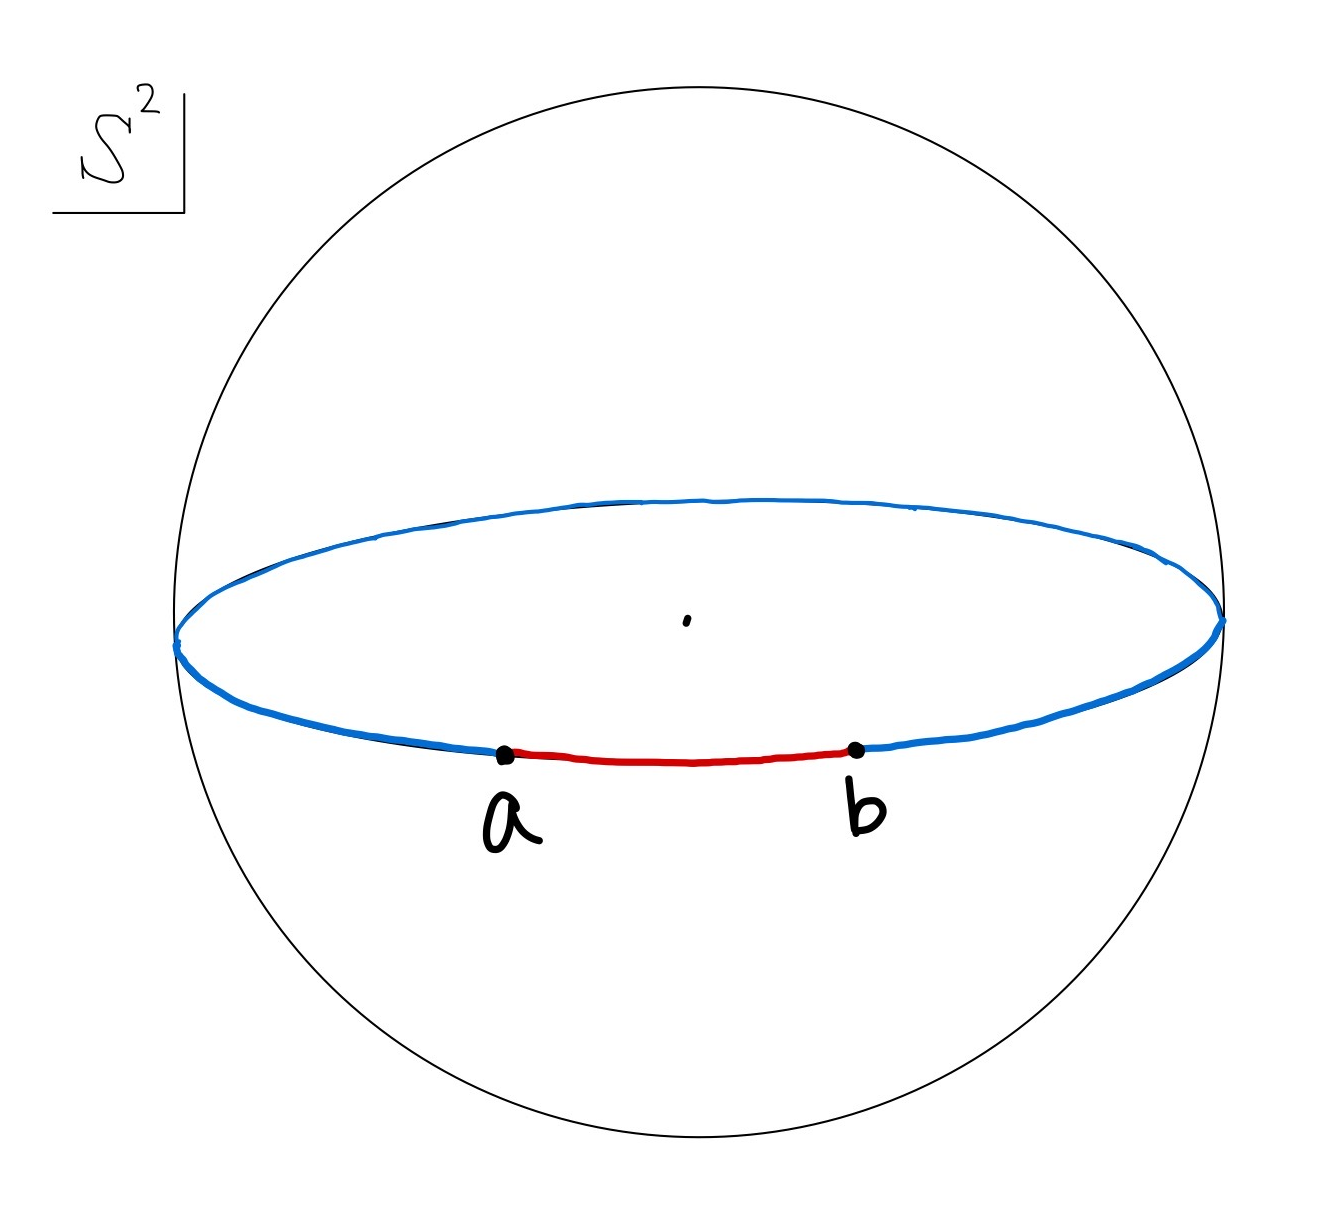
\includegraphics{mensetsu-sokuchisen.png}}
\end{center}
\(a\)と\(b\)を結ぶ測地線は2つある.
\vspace{10pt}

\raisebox{-0.5mm}[0mm]{
\includegraphics[bb=0 0 150 30, scale=0.5]{yokoyazirushi.png}} \hspace{-40pt}
リーマン多様体において,
\begin{table}
      \vspace{0pt}
      \begin{tabular}{lll}
      2点間を結ぶ曲線で長さが最短であるもの
      & \(\Rightarrow\)
      & 測地線\\
      & \textcolor{red}{\(\centernot\Leftarrow\)}
      &
      \end{tabular}
      \vspace{-8pt}
\end{table}
\hspace{190pt}\textcolor{red}{一般に言えない!}
}




\frame{
\frametitle{\insertsection}
\underline{球面における三角形}
\begin{table}
      \begin{tabular}{lll}
      三角形
      & \(\overset{\mathrm{def}}{\Leftrightarrow}\)
      & 3つの測地線によって囲まれたコンパクト閉領域
      \end{tabular}
\end{table}
\begin{center}
\scalebox{0.1}{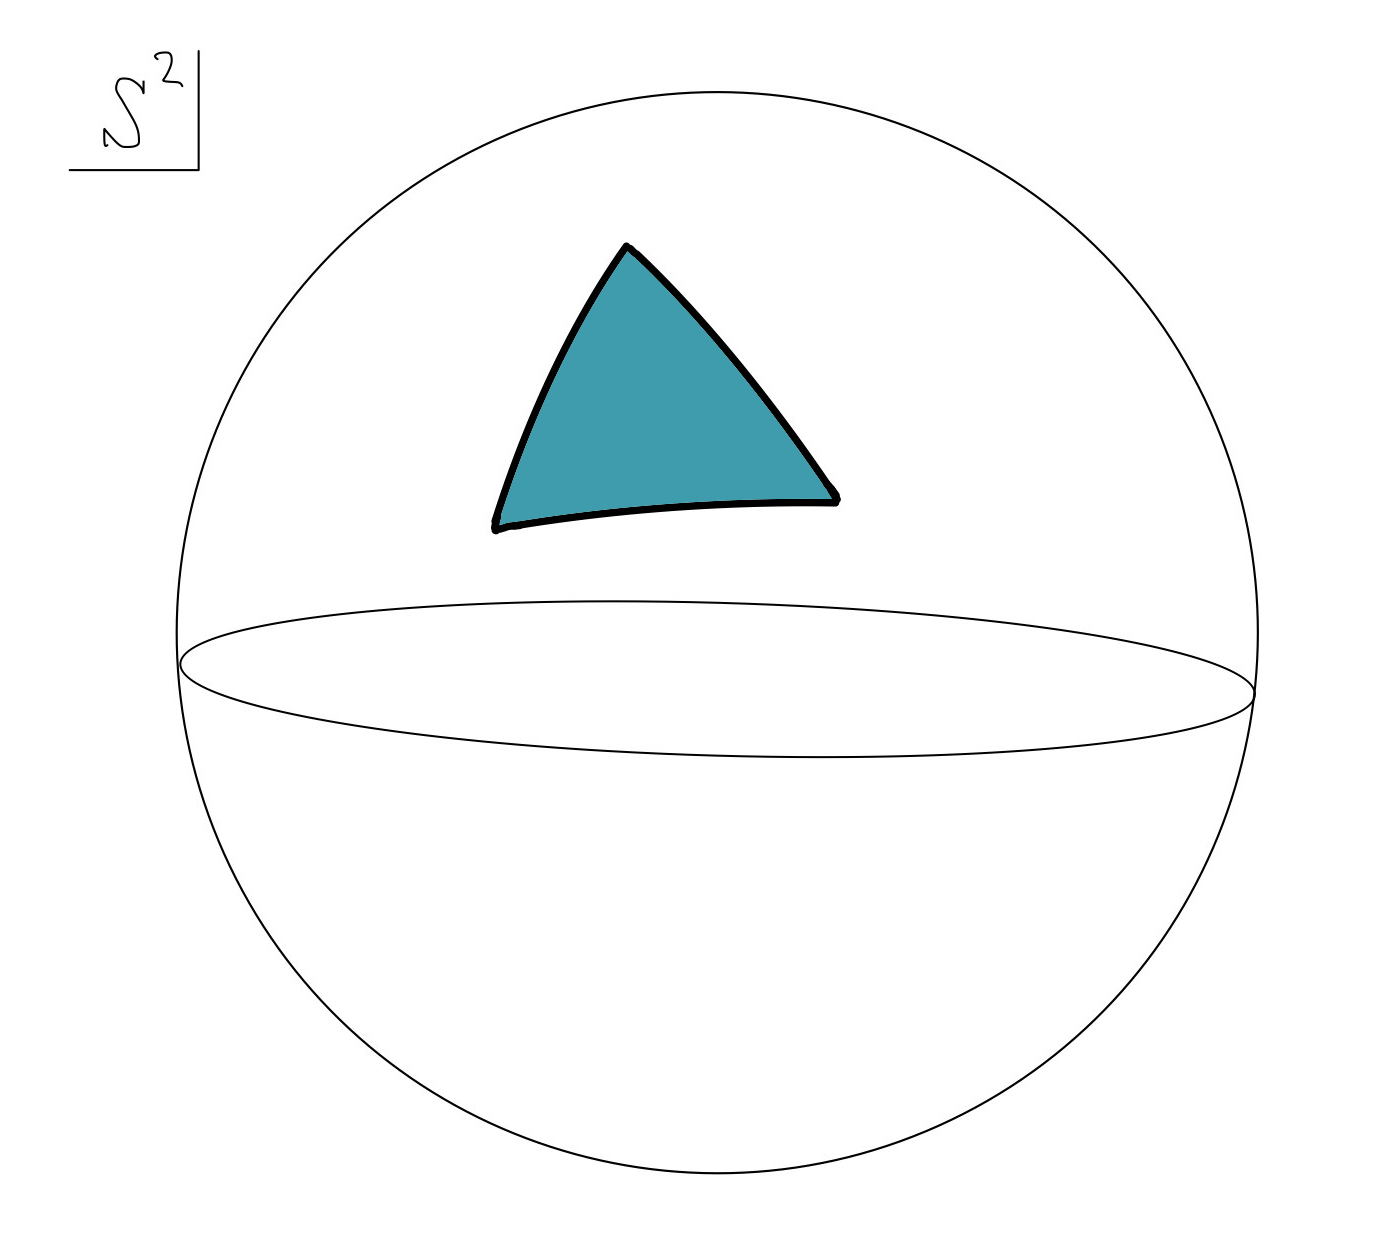
\includegraphics{mensetsu-sankaku1.png}}
\pause
\scalebox{0.1}{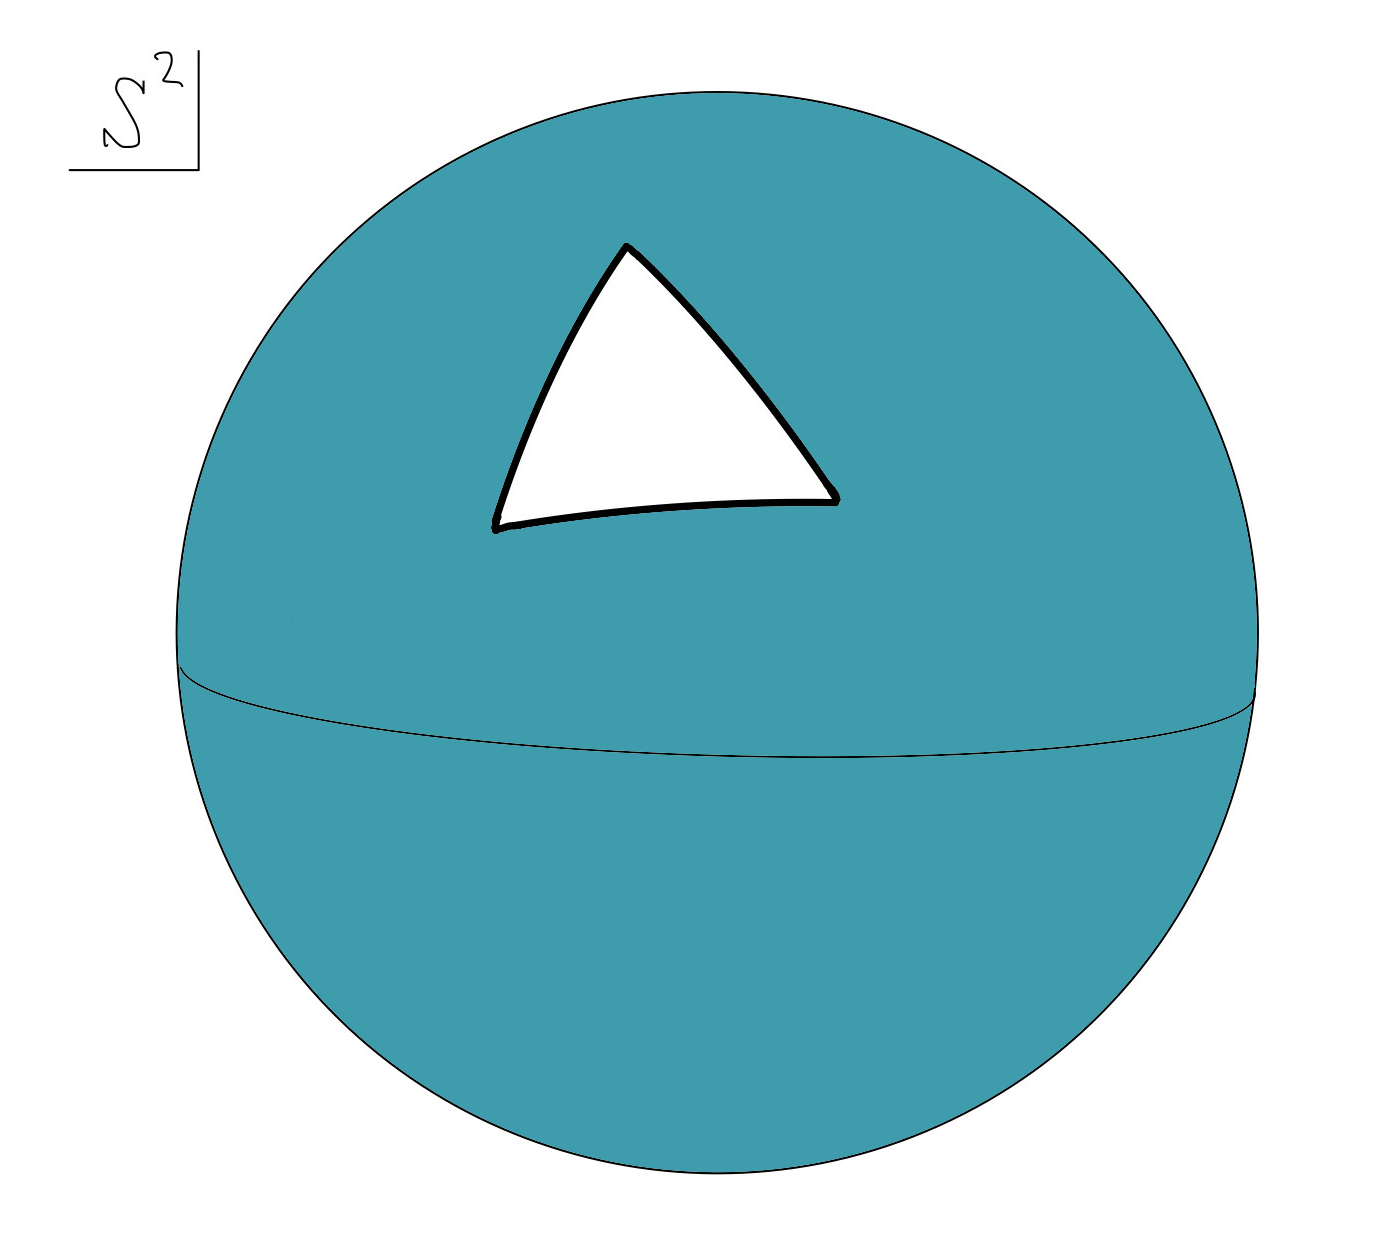
\includegraphics{mensetsu-sankaku2.png}}
\end{center}
\pause
また,リーマン多様体では,三角形の内角の和が\(180^\circ\)とは限らない!
}


% \section{おまけ:擬リーマン多様体における測地線}
% \frame{
% \frametitle{\insertsection}
% \hspace{3pt}\(M\) \hspace{4pt}: \(C^\infty\)多様体 
% \vspace{3pt}

% \(TM\) : \(M\)の接空間
% \vspace{3pt}

% \( X, Y \,\in TM\)
% \vspace{3pt}

% \(g : TM \times TM \rightarrow \mathbb{R}\)
% \vspace{3pt}
% \begin{table}
% \begin{tabular}{rlcl}
% \hspace{-10pt}\(g\) : \(M\)上のリーマン計量
% & \(\overset{\mathrm{def}}{\Leftrightarrow}\)
% & (\rnum{1})& \(g\) : 多重双線型
% \\
% & & (\rnum{2})& \(g( X, Y)=g(Y, X)\)(対称)
% \\
% & &
% (\rnum{3})& \(g(X, X)\geq 0\) かつ\\
% & & &\(g(X, X)=0\Leftrightarrow X=0\)(正定値)
% \end{tabular}
% \vspace{5pt}
% \pause

% \begin{tabular}{rlcl}
% \hspace{-8pt}\(g\) : \textcolor{red}{{\it \(M\)上の擬リーマン計量}}
% & \(\overset{\mathrm{def}}{\Leftrightarrow}\)
% & (\rnum{1})& \(g\) : 多重双線型
% \\
% & & (\rnum{2})& \(g( X, Y)=g(Y, X)\)(対称)
% \pause
% \\
% & &
% \textcolor<3->{red}{(\rnum{3})}& \textcolor<3->{red}{\(g(X, Y)=0 \,\, (^\forall Y) \Rightarrow X=0\)(非退化)}
% \end{tabular}
% \end{table}
% \begin{center}
% {\bf \underline{{\large 一般相対性理論における時空は擬リーマン多様体!}}}
% \end{center}
% }



% \frame{
% \frametitle{\insertsection}
% \((M, g)\) : 擬リーマン多様体
% \begin{defi}
% \(X \in TM\)
%       \begin{table}
%       \vspace{-5pt}
%       \begin{center}
%       \begin{tabular}{lllcl}
%       $X$ : \textcolor{red}{{\it spacelike}} & 
%       $\overset{\mathrm{def}}{\Leftrightarrow}$ &
%       $g(X, X) >0$ &
%       or &
%       $X=0$
%       \\
%       $X$ : \textcolor{red}{{\it timelike}} & 
%       $\overset{\mathrm{def}}{\Leftrightarrow}$ & 
%       $g(X, X) <0$ & 
%       \\
%       $X$ : \textcolor{red}{{\it null}} & 
%       $\overset{\mathrm{def}}{\Leftrightarrow}$ &
%       $g(X, X) =0$ &
%       and &
%       $X\neq 0$
%       \end{tabular}
%       \end{center}
%       \vspace{-10pt}
%       \end{table}
% \begin{center}
% \(M\)上の曲線\(c\)が\textcolor{red}{null曲線} \quad
% \(\overset{\mathrm{def}}{\Leftrightarrow}\) \quad
% 速度ベクトル\(\dot{c}\)がnullベクトル
% \end{center}
% \pause
% \vspace{0pt}
% \end{defi}
% \vspace{10pt}
% \begin{center}
% {\bf \underline{{\large 時空における光の粒子の軌跡はnull測地線!}}}
% \end{center}
% }

\end{document}